\chapter{RTS AI: \textit{StarCraft: Broodwar}}

\section{How does the game works: gameplay}
Really, the best is to play it... But I'll explain it.

In combinatorial game theory terms, competitive StarCraft is a zero sum, partial-information, deterministic strategy game.

\section{Problems, resolutions}

\begin{figure}[!ht]
\begin{center}
\begin{tikzpicture}
  \path[mindmap,concept color=black!80!white,text=white]
    node[concept] {RTS AI: predict, decide, perform}
    [clockwise from=-30]
    child[concept color=orange!90!black] {
      node[concept] {Micro}
      child[concept color=red!80!magenta] { node[concept] {React} }
      child { node[concept] {Optimize} }
      child[concept color=blue!80!cyan] { node[concept] {Cooperate} }
    }
    child[concept color=cyan!90!black] { % TODO change color
      node[concept] {Tactics}
      child[concept color=red!80!magenta] { node[concept] {When?} }
      child { node[concept] {Where?} }
      child[concept color=blue!80!cyan] { node[concept] {How?} }
    }
    child[concept color=green!70!black] {
      node[concept] {Strategy}
      child[concept color=red!80!magenta] { node[concept] {Aggressivity} }
      child { node[concept] {Spendings balance} }
      child[concept color=blue!80!cyan] { node[concept] {Army composition} }
    };  
\end{tikzpicture}
\end{center}
\label{fig:mindmapRTS}
\caption{A mind-map of RTS AI XXX TODO}
\end{figure}

\section{Task decomposition and linking}
\begin{figure}[!ht]
\begin{center}
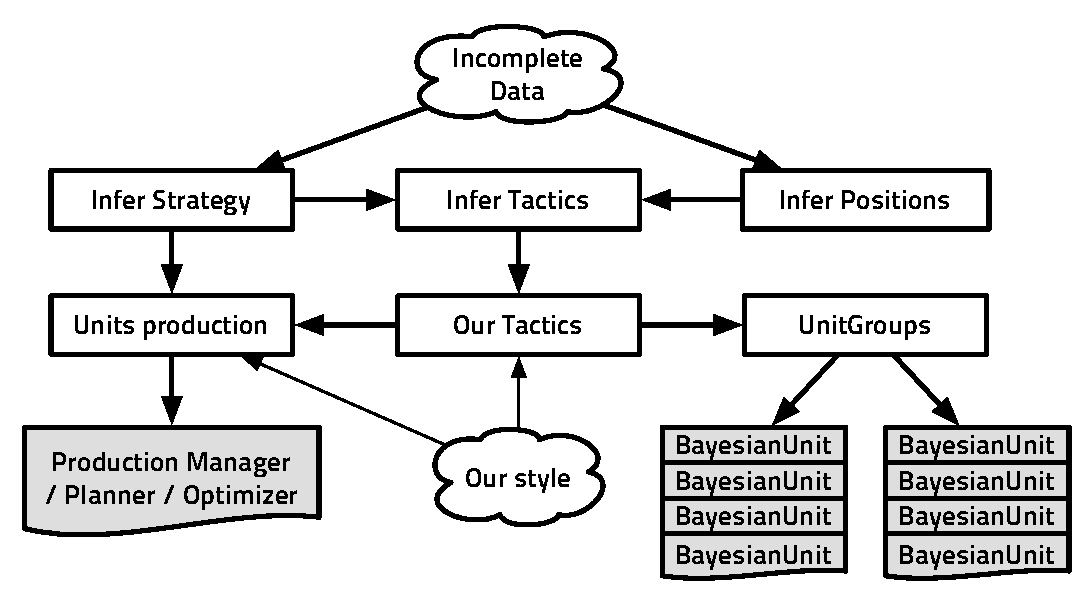
\includegraphics[width=13cm]{images/starcraft_bbq_concept_12-04-2012.pdf}
\end{center}
\label{fig:conceptbbq}
\caption{Information-centric view of the architecture of the bot, the gray parts perform game actions (as the physical actions of the player on the keyboard and mouse).}
\end{figure}

In Fig.~\ref{fig:conceptbbq}, we present the flow of informations between the different inference and decision-making parts of the bot architecture. One can also view this problem as having a good model of one's strategy, one's opponent strategy, and taking decisions. The software architecture that we propose is to have services building and maintaining the model of the enemy as well as our state, and decision-making modules using all this information to give orders to actuators.

\begin{itemize}
\item Problem: build a real-scale software piece which is maintainable
\item State of the art: shared memories, shared states
\item Our take: we transmit distributions, states stay in modules
\item Results: XXX (atm too much state), also competitions results
\end{itemize}
